\section{Пример III}
Задана ЗЛП:
$$F(\vec{X}) = x_1+4x_2 \to max$$
\begin{equation}
\label{system}
\begin{cases}
2x_1+4x_2 \le 17\\
10x_1+3x_2 \le 15\\
x_i \ge 0 \\
\end{cases}
\end{equation}

\subsection{Решение исходной ЗЛП}
Введем искусственные переменные и приведем к каноническому виду.
Для нахождения максимума, умножим целевую функцию на -1.

$$-F(\vec{X}) = -(-x_1-4x_2) \to max$$
\begin{equation}
\label{cannonical}
\begin{cases}
2x_1+4x_2+x_3=17\\
10x_1+3x_2+x_4=15\\
x_i, s_i \ge 0 \\
\end{cases}
\end{equation}

\begin{center}
\begin{tabular*}{\textwidth}{@{\extracolsep{\fill}}|c|c|c|c|c|c|c|c|c|}
\hline
$i$ & Базис & $C_i$ & B & $C_1 = -1$ & $C_2 = -4$ & $C_3 = 0$ & $C_4 = 0$ & $\Theta_i$ \\
\hline
$1$ & $P_3$ & $0$ & $17$ & $2$ & $4$ & $1$ & $0$ & $4,25$\\
$2$ & $P_4$ & $0$ & $15$ & $10$ & $3$ & $0$ & $1$ & $5$\\
\hline
$m+1$ & ~ & ~ & $0$ & $1$ & $4$ & $0$ & $0$ & ~ \\
\hline
\end{tabular*}
\end{center}
\begin{center}
\begin{tabular*}{\textwidth}{@{\extracolsep{\fill}}|c|c|c|c|c|c|c|c|c|}
\hline
$i$ & Базис & $C_i$ & B & $C_1 = -1$ & $C_2 = -4$ & $C_3 = 0$ & $C_4 = 0$ & $\Theta_i$ \\
\hline
$1$ & $P_2$ & $-4$ & $4,25$ & $0,5$ & $1$ & $0,25$ & $0$ & $4,25$\\
$2$ & $P_4$ & $0$ & $2,25$ & $8,5$ & $0$ & $-0,75$ & $1$ & $5$\\
\hline
$m+1$ & ~ & ~ & $-17$ & $0$ & $0$ & $-1$ & $0$ & ~ \\
\hline
\end{tabular*}
\end{center}
Получен оптимальный план: $X^{опт} = (0;4,25)$, и оптимальное значение целевой функции $F^{опт} = 17$.

\subsection{Нахождение целочисленных решений}
Компонент $P_2$ полученного плана не является целочисленным. Применим алгоритм Гомори.
Первое отсечение:
\begin{equation}
-0,5 x_1 - 0,25 x_3 + U_1 = -0,25.
\end{equation}
\begin{center}
\begin{tabular*}{\textwidth}{@{\extracolsep{\fill}}|c|c|c|c|c|c|c|c|c|c|}
\hline
$i$ & Базис & $C_i$ & B & $C_1 = -1$ & $C_2 = -4$ & $C_3 = 0$ & $C_4 = 0$ & $C_5 = 0$ & $\Theta_i$ \\
\hline
$1$ & $P_2$ & $-4$ & $4,25$ & $0,5$ & $1$ & $0,25$ & $0$ & $0$ & --\\
$2$ & $P_4$ & $0$ & $2,25$ & $8,5$ & $0$ & $-0,75$ & $1$ & $0$ & --\\
$3$ & $P_5$ & $0$ & $-0,25$ & $-0,5$ & $0$ & $-0,25$ & $0$ & $1$ & --\\
\hline
$m+1$ & ~ & ~ & $-17$ & $0$ & $0$ & $0$ & $0$ & $0$ & ~ \\
\hline
\end{tabular*}
\end{center}
\begin{center}
\begin{tabular*}{\textwidth}{@{\extracolsep{\fill}}|c|c|c|c|c|c|c|c|c|c|}
\hline
$i$ & Базис & $C_i$ & B & $C_1 = -1$ & $C_2 = -4$ & $C_3 = 0$ & $C_4 = 0$ & $C_5 = 0$ & $\Theta_i$ \\
\hline
$1$ & $P_2$ & $-4$ & $4$ & $0$ & $1$ & $0$ & $0$ & $1$ & --\\
$2$ & $P_4$ & $0$ & $-2$ & $0$ & $0$ & $-5$ & $1$ & $17$ & --\\
$3$ & $P_1$ & $-1$ & $0,5$ & $1$ & $0$ & $0,5$ & $0$ & $-2$ & --\\
\hline
$m+1$ & ~ & ~ & $-17$ & $0$ & $0$ & $0$ & $0$ & $0$ & ~ \\
\hline
\end{tabular*}
\end{center}
Второе отсечение:
\begin{equation}
- 0,5 x_3  + U_2 = -0,5.
\end{equation}
\begin{center}
\begin{tabular*}{\textwidth}{@{\extracolsep{\fill}}|c|c|c|c|c|c|c|c|c|c|c|}
\hline
$i$ & Базис & $C_i$ & B & $C_1 = -1$ & $C_2 = -4$ & $C_3 = 0$ & $C_4 = 0$ & $C_5 = 0$ & $C_6 = 0$ & $\Theta_i$ \\
\hline
$1$ & $P_2$ & $-4$ & $4$ & $0$ & $1$ & $0$ & $0$ & $1$ & $0$ & --\\
$2$ & $P_4$ & $0$ & $-2$ & $0$ & $0$ & $-5$ & $1$ & $17$ & $0$ & --\\
$3$ & $P_1$ & $-1$ & $0,5$ & $1$ & $0$ & $0,5$ & $0$ & $-2$ & $0$ & --\\
$4$ & $P_6$ & $0$ & $-0,5$ & $0$ & $0$ & $-0,5$ & $0$ & $0$ & $1$ & --\\
\hline
$m+1$ & ~ & ~ & $-17$ & $0$ & $0$ & $0$ & $0$ & $0$ & $0$ & ~ \\
\hline
\end{tabular*}
\end{center}
\begin{center}
\begin{tabular*}{\textwidth}{@{\extracolsep{\fill}}|c|c|c|c|c|c|c|c|c|c|c|}
\hline
$i$ & Базис & $C_i$ & B & $C_1 = -1$ & $C_2 = -4$ & $C_3 = 0$ & $C_4 = 0$ & $C_5 = 0$ & $C_6 = 0$ & $\Theta_i$ \\
\hline
$1$ & $P_2$ & $-4$ & $4$ & $0$ & $1$ & $0$ & $0$ & $1$ & $0$ & --\\
$2$ & $P_4$ & $0$ & $3$ & $0$ & $0$ & $0$ & $1$ & $17$ & $-10$ & --\\
$3$ & $P_1$ & $-1$ & $0$ & $1$ & $0$ & $0$ & $0$ & $-2$ & $1$ & --\\
$4$ & $P_3$ & $0$ & $1$ & $0$ & $0$ & $1$ & $0$ & $0$ & $-2$ & --\\
\hline
$m+1$ & ~ & ~ & $-17$ & $0$ & $0$ & $0$ & $0$ & $0$ & $0$ & ~ \\
\hline
\end{tabular*}
\end{center}
Получен оптимальный план: $X^{опт} = (0;4)$, и оптимальное значение целевой функции $F^{опт} = 16$.

\newpage
\subsection{Решение ЗЛП в программе}
Введем ЗЛП в программу и сравним результаты.

\begin{figure}[hb]
\centering
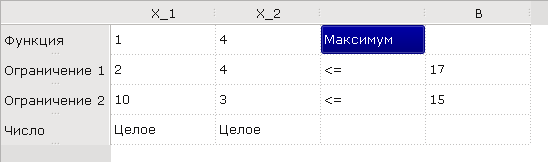
\includegraphics[scale=1.0]{img/problem31.png}
\caption{Условие задачи в программе}
\end{figure}

\begin{figure}[ht]
\centering
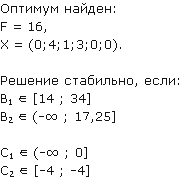
\includegraphics[scale=1.0]{img/solution31.png}
\caption{Решение задачи в программе}
\end{figure}
